\documentclass[border=12pt]{standalone}
\usepackage{tikz}
\usetikzlibrary{positioning, arrows.meta, fit, backgrounds, calc}

\begin{document}
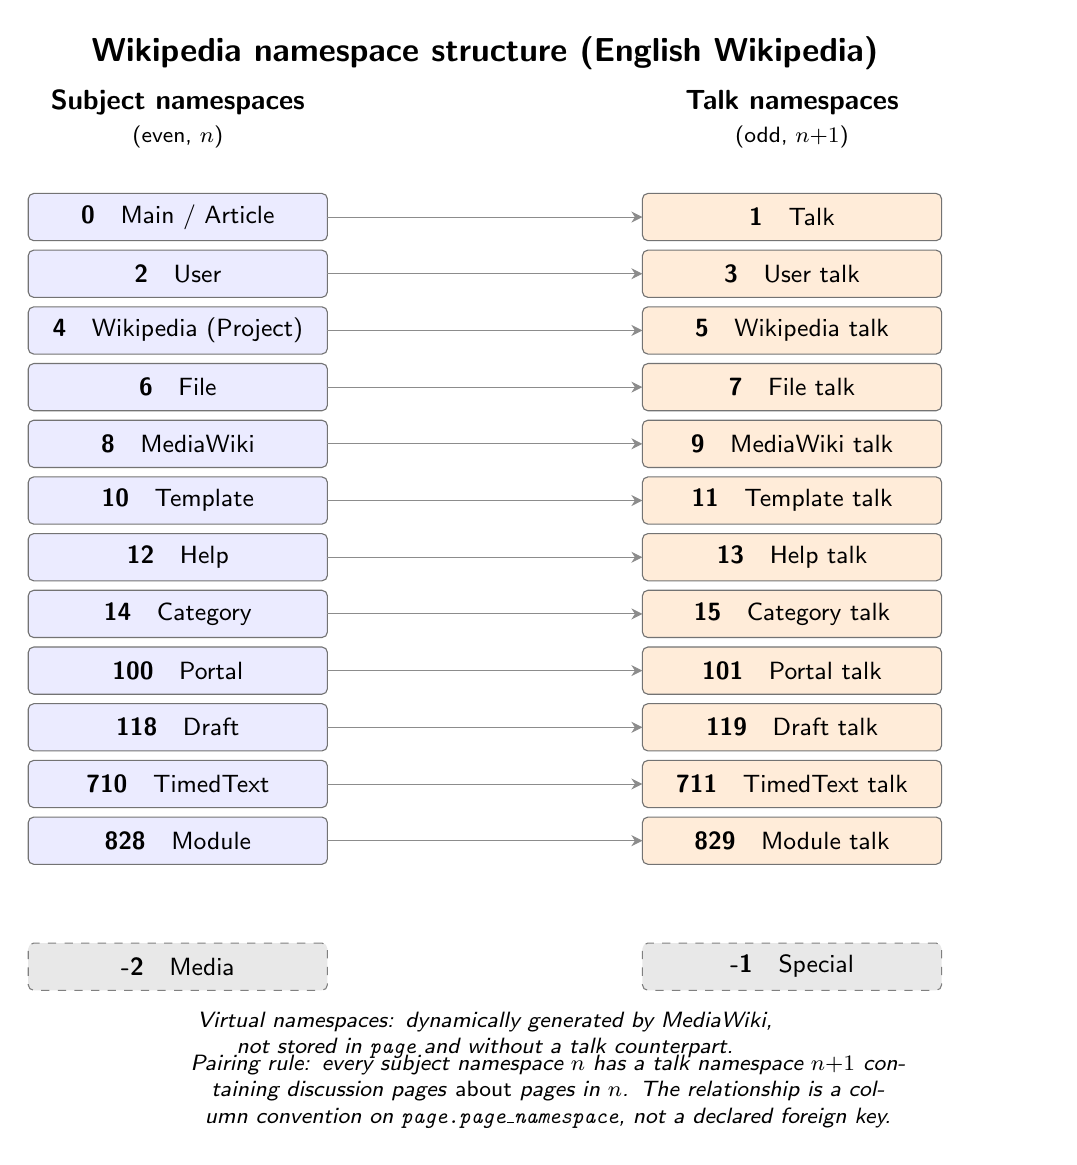
\begin{tikzpicture}[
    font=\sffamily\small,
    ns/.style={
        rectangle, rounded corners=2pt,
        draw=black!55, line width=0.4pt,
        minimum width=3.8cm, minimum height=0.6cm,
        align=left, inner sep=4pt, outer sep=0pt,
    },
    subject/.style={ns, fill=blue!8},
    talk/.style={ns, fill=orange!15},
    virtual/.style={ns, fill=gray!18, draw=black!50, dashed},
    pair/.style={-{Stealth[length=4pt, width=4pt]}, draw=black!45, line width=0.35pt},
    header/.style={
        font=\sffamily\bfseries,
        align=center, minimum width=3.8cm,
    },
    title/.style={font=\sffamily\bfseries\large, align=center},
    note/.style={font=\sffamily\itshape\footnotesize, align=center},
]

% --- Subject (even) column ---
\node[subject] (s0)   {\textbf{0}\quad Main / Article};
\node[subject, below=0.12cm of s0]   (s2)   {\textbf{2}\quad User};
\node[subject, below=0.12cm of s2]   (s4)   {\textbf{4}\quad Wikipedia (Project)};
\node[subject, below=0.12cm of s4]   (s6)   {\textbf{6}\quad File};
\node[subject, below=0.12cm of s6]   (s8)   {\textbf{8}\quad MediaWiki};
\node[subject, below=0.12cm of s8]   (s10)  {\textbf{10}\quad Template};
\node[subject, below=0.12cm of s10]  (s12)  {\textbf{12}\quad Help};
\node[subject, below=0.12cm of s12]  (s14)  {\textbf{14}\quad Category};
\node[subject, below=0.12cm of s14]  (s100) {\textbf{100}\quad Portal};
\node[subject, below=0.12cm of s100] (s118) {\textbf{118}\quad Draft};
\node[subject, below=0.12cm of s118] (s710) {\textbf{710}\quad TimedText};
\node[subject, below=0.12cm of s710] (s828) {\textbf{828}\quad Module};

% --- Talk (odd) column, paired row-by-row ---
\node[talk, right=4cm of s0]   (t1)   {\textbf{1}\quad Talk};
\node[talk, right=4cm of s2]   (t3)   {\textbf{3}\quad User talk};
\node[talk, right=4cm of s4]   (t5)   {\textbf{5}\quad Wikipedia talk};
\node[talk, right=4cm of s6]   (t7)   {\textbf{7}\quad File talk};
\node[talk, right=4cm of s8]   (t9)   {\textbf{9}\quad MediaWiki talk};
\node[talk, right=4cm of s10]  (t11)  {\textbf{11}\quad Template talk};
\node[talk, right=4cm of s12]  (t13)  {\textbf{13}\quad Help talk};
\node[talk, right=4cm of s14]  (t15)  {\textbf{15}\quad Category talk};
\node[talk, right=4cm of s100] (t101) {\textbf{101}\quad Portal talk};
\node[talk, right=4cm of s118] (t119) {\textbf{119}\quad Draft talk};
\node[talk, right=4cm of s710] (t711) {\textbf{711}\quad TimedText talk};
\node[talk, right=4cm of s828] (t829) {\textbf{829}\quad Module talk};

% --- Pairing arrows: subject n  ->  talk n+1 ---
\foreach \s/\t in {%
    s0/t1, s2/t3, s4/t5, s6/t7, s8/t9, s10/t11,
    s12/t13, s14/t15, s100/t101, s118/t119, s710/t711, s828/t829%
}{
    \draw[pair] (\s.east) -- (\t.west);
}

% --- Column headers, aligned to their columns ---
\node[header, above=0.45cm of s0]   (hsubj) {Subject namespaces \\ \footnotesize\mdseries (even, $n$)};
\node[header, above=0.45cm of t1]   (htalk) {Talk namespaces \\ \footnotesize\mdseries (odd, $n{+}1$)};

% --- Title ---
\node[title, above=0.5cm of $(hsubj)!0.5!(htalk)$]
    {Wikipedia namespace structure (English Wikipedia)};

% --- Virtual namespaces (no stored pages, no talk pair) ---
\node[virtual, below=1.0cm of s828.south, xshift=0cm] (sm2) {\textbf{-2}\quad Media};
\node[virtual, right=4cm of sm2] (sm1) {\textbf{-1}\quad Special};

\node[note, below=0.15cm of $(sm2.south)!0.5!(sm1.south)$, text width=10cm]
    {Virtual namespaces: dynamically generated by MediaWiki, \\
     not stored in \texttt{page} and without a talk counterpart.};

% --- Footnote / legend ---
\node[note, below=0.7cm of sm2.south, xshift=4.7cm, text width=12.5cm] (legend)
    {Pairing rule: every subject namespace $n$ has a talk namespace $n{+}1$
     containing discussion pages \emph{about} pages in $n$.
     The relationship is a column convention on \texttt{page.page\_namespace},
     not a declared foreign key.};

\end{tikzpicture}
\end{document}
